%======================	%
%	LaTeX SETUP			%
%======================	%
\documentclass[portrait]{scrreprt}						% Change "article" to "report" to get rid of page number on title page
\usepackage{amsmath,amsfonts,amsthm,amssymb,empheq,setspace,Tabbing,fancyhdr,lastpage,extramarks,chngpage,soul,color,graphicx,float,wrapfig,lscape}
\usepackage[retainorgcmds]{IEEEtrantools}
%======================	%
%	TikZ SETUP			%
%======================	%
\usepackage{tikz,verbatim}
\usetikzlibrary{shapes,arrows,positioning,calc,scopes,angles,quotes,decorations.markings}
%======================	%
%	MARGINS				%
%======================	%
\topmargin=-0.45in      
\evensidemargin=0in     
\oddsidemargin=0in      
\textwidth=6.5in        
\textheight=9.0in       
\headsep=0.25in         
%======================	%
%	HEADER/FOOTER		%
%======================	%
                                
%======================	%
%	MATH COMMANDS		%
%======================	%
	%creates roman-script differential d, with added space
\newcommand{\ud}{\,\mathrm{d}}
	%partial derivative
\newcommand{\pd}[2]{\frac {\partial #1}{\partial #2}}
	%derivative
\newcommand{\td}[2]{\frac {\mathrm{d} #1}{\mathrm{d} #2}}
	%second derivative
\newcommand{\tdd}[2]{\frac {\mathrm{d}^2 #1}{\mathrm{d} #2^2}}
	%formats a numerical value with text units
\newcommand{\val}[2]{#1 \text{ #2}}
	%comment for IEEE aligned environment
\newcommand{\comm}[1]{\text{#1}\qquad}

%======================	%
%	BEGIN DOCUMENT		%
%======================	%
\begin{document}



�
\centering

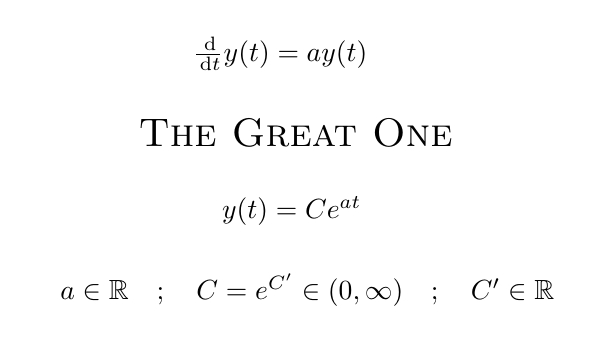
\begin{tikzpicture}

\draw (0,2) node{$\frac{\ud{}}{\ud{t}}y(t)  =ay(t)\phantom{\frac{\ud{}}{\ud{t}}} $};
\draw (0,1) node{{\Large\textsc{The  Great One}}};
\draw (0,0) node{$y(t) = Ce^{at}\phantom{.} $};
\draw (0,-1) node{$\phantom{x.}a \in \mathbb{R} \quad;\quad C=e^{C'} \in (0,\infty)\quad;\quad C' \in \mathbb{R}  $};




\end{tikzpicture}

\end{document}

\begin{IEEEeqnarray*}{rCl}
z & = & Z' \\
y & = & Y \\
\end{IEEEeqnarray*}



















